\subsection{Line Integrals}
Why do vector fields matter? What can we do with them? Consider the classic physics example of work done lifting an object. When near the surface of the earth, gravity is nearly constant, so the elementary formula work equals force times distance can be used simply. However, if we are lifting an object with varying mass or moving an object very far away from the surface of the earth we need to apply an integral to account for the changing forces. To add even another level of complexity, if you consider something like a rocket going into orbit, we can compute the amount of work by modeling the gravitational forces as a vector field and integrating across a path through said vector field. These types of integrals, where we integrate a vector field over some line, are called \textbf{line integrals}.

\begin{definition}{Line Integrals}
Let $C$ be a smooth curve in $\bbr^n$ of finite length parameterized by $$r(t), \ a\leq t\leq b.$$ Let $\vcT$ be the unit tangent vector to $\vcr(t)$. Let $\vcF$ be a vector field  $\bbr^n\to\bbr^n$. Then the line integral of $\vcF$ over $C$ is the integral of the projection of $\vcF$ onto $\vcT$ at each point along $C$, that is, $$\int_C \vcF \ d\vcr=\int_C \proj{\vcF}{\vcT} \ ds.$$
This line integral can be evaluated 
$$\int_C \proj{\vcF}{\vcT} \ ds=\int_a^b \vcF(\vcr(t))\bullet\vcr\vprime(t)\ dt.$$
\end{definition}

\begin{example}{\hypertarget{ftli}{Line Integrals}}
Consider the vector field $$\vcF=\bmat{y+1\\x} $$ and the curve $C$ parameterized by $$\vcr(t)=\bmat{\cos(t)\\ \sin(t)}, \ 0\leq t\leq\pi/2. $$
Then the line integral can be computed as 
\begin{align*}
\int_C \vcF \ d\vcr=&\int_{0}^{\pi/2}\vcF(\vcr(t))\bullet\vcr\vprime(t)\ dt\\
=&\int_{0}^{\pi/2}\bmat{\sin(t)+1\\ \cos(t)}\bullet\bmat{-\sin(t)\\\cos(t)}\ dt\\
=&\int_{0}^{\pi/2}-\sin^2(t)-\sin(t)+\cos^2(t)\ dt\\
=&\int_{0}^{\pi/2}\cos(2t)-\sin(t)\ dt\\
=&\Bigg[\frac{\sin(2t)}{2}+\cos(t)\Bigg]_{t=0}^{t=\pi/2}\\
=&\frac{\sin(\pi)}{2}+\cos(\pi/2)-\left(\frac{\sin(0)}{2}+\cos(0)\right)\\
=& 0+0-(0+1)\\
=&-1.
\end{align*}
The vector field and curve that we integrated over are graphed below-- note that our curve is oriented counterclockwise.
\vspace{1em}
\begin{center}
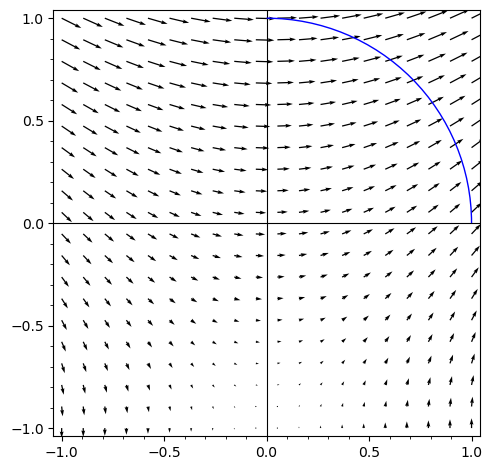
\includegraphics[scale=0.5]{Figures/lineintex}\\
Vector field and Curve (in blue).
\end{center}
\end{example}

\begin{exercise}{Doing It Backwards}
Take the same vector field and curve, but this time orient the curve clockwise. That is, let $$\vcF=\bmat{y+1\\x} $$ as before, but let $$\vcr(t)=\bmat{\sin(t)\\ \cos(t)}, \ 0\leq t\leq \pi/2$$ instead. Note: Our previous parameterization went from $(1,0)$ at $t=0$ to $(0,1)$ at $t=\pi/2$, while this parameterization goes from $(0,1)$ at $t=0$ to $(1,0)$ at $t=\pi/2$.
\end{exercise}

\begin{pexercise}{3 Dimensional}
Let $$\vcF=\bmat{8x^2yz\\5z\\-4xy}$$ and let $C$ be the curve parameterized by $$C=\left\{\vcr(t):\ \vcr(t)=\bmat{t\\t^2\\t^3},\ 0\leq t\leq 1\right\}. $$ Find $$\int_C \vcF \ dr.$$
\end{pexercise}

An important application of line integrals is finding the work it takes to move an object through a vector field. 

\begin{example}{Physics and non-parameterized curves}
Let $$\vcF=\bmat{5y\\10x}$$ and $$c=\left\{\vcr(t):\ \vcr(t)=\bmat{t\\ t^2/2},\ 0\leq t\leq 2 \right\}.$$
Then the work is equal to the line integral of $c$ over $\vcF$, or $$\int_C \vcF \ d\vcr. $$
We can evaluate this as 
\begin{align*}
\int_C\vcF \ d\vcr=&\int_0^2 \vcF(\vcr(t))\bullet\vcr\vprime(t)\ dt \\
=&\int_0^2 \bmat{5\left(t^2/2\right)\\10(t)}\bullet\bmat{1\\t}\ dt\\
=&\int_0^2\bmat{2.5t^2\\10t}\bullet\bmat{1\\ t} \ dt\\
=&\int_0^2 (2.5t^2)(1)+(10t)(t)\ dt\\
=&\int_0^2 12.5t^2\ dt\\
=&12.5\frac{t^3}{3}\Bigg]_0^2\\
=&\frac{100}{3}.
\end{align*}

\end{example}